\documentclass[10pt,twocolumn,letterpaper]{article}

\usepackage[pagenumbers]{cvpr}

\usepackage{graphicx}
\usepackage{amsmath}
\usepackage{amssymb}
\usepackage{booktabs}
\usepackage[pagebackref,breaklinks,colorlinks]{hyperref}
\usepackage[capitalize]{cleveref}
\crefname{section}{Sec.}{Secs.}
\Crefname{section}{Section}{Sections}
\Crefname{table}{Table}{Tables}
\crefname{table}{Tab.}{Tabs.}

\begin{document}

\title{Paper Review and Notes For\\BEIT: BERT Pre-Training of Image Transformers}

\author{Jin Hyoung Joo\\ {\tt\small hyoungjoo.j@gmail.com} }
\maketitle

\begin{abstract}
    This paper \cite{BEIT} introduces \emph{BEIT} (Bidirectional Encoder representation
    from Image Transformers), which is a self-supervised vision model that is trained
    by the proposed masked image modeling task.
\end{abstract}

\begin{figure}[ht]
  \centering
   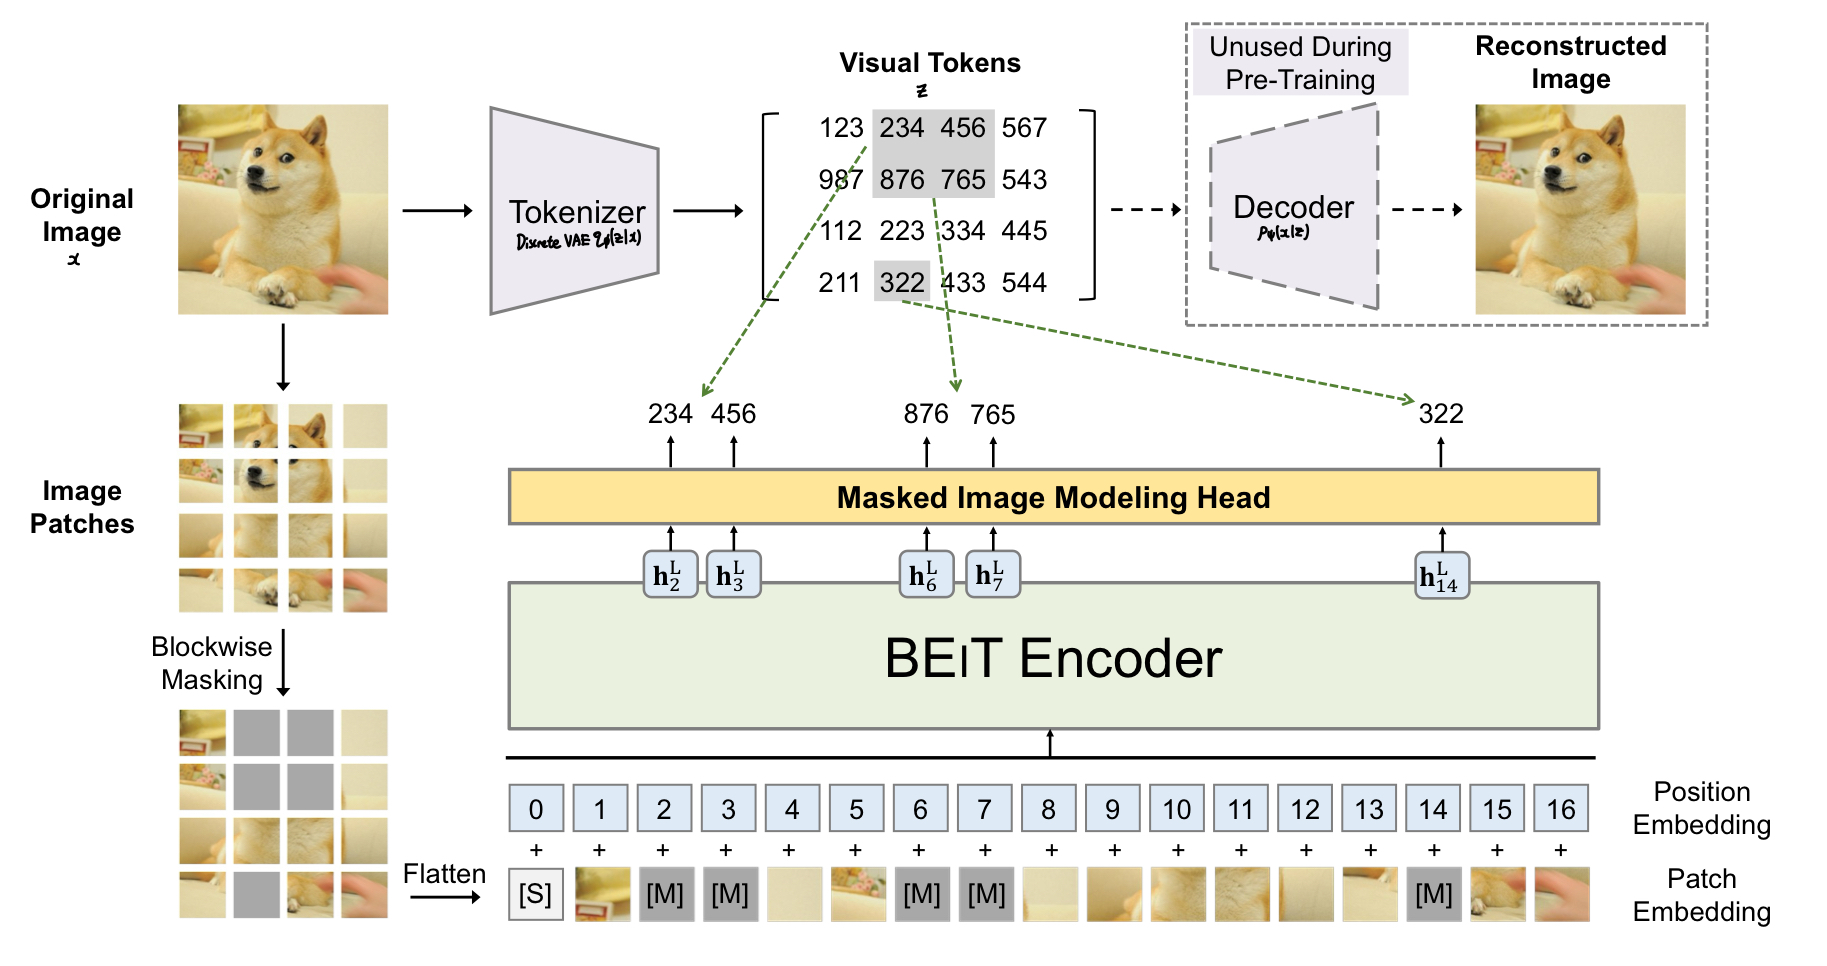
\includegraphics[width=\linewidth]{figures/model-architecture.jpeg}
   \caption{Model architecture of BEIT.}
\end{figure}

\section{Key Points}
\subsection{Background of BEIT}
Even though Vision Transformers are performant, they require large amounts of training data.
To solve this problem, self-supervised pre-training is neccessary.

BERT achieved great success in NLP using the masked language modeling task, which is to predict
the masked tokens of a given text based on the Transformer's encoding results.
Naively applying this method to Vision Transformers have the following problems.
\begin{itemize}
    \item{There is no pre-existing vocabulary for image patches.}
    \item{Pixel-level recovery tasks waste modeling capabilities on pre-training short-range dependencies
        and high-frequency details.}
\end{itemize}

\subsection{Proposed Method}
The pre-training of BEIT operates in the following steps.
\begin{enumerate}
    \item{The image is split into a grid of patches.}
    \item{Using a pre-trained discrete VAE, the image is tokenized into discrete visual tokens.}
    \item{Some proportion of the image patches are masked, and the corrupted input is used as input to the Transformer.}
    \item{The model learns to recover the visual tokens of the original image (output of Step 2).}
\end{enumerate}

\subsection{Advantages of BEIT}
BEIT has improved convergence speed, high stability, and lower training costs on end tasks.
A self-supervised BEIT can also learn reasonable semantic regions via pre-training even with
no human supervision.

\section{Technical Details}
\subsection{Blockwise Masking}
\subsection{Training Objective}
\section{Further Research}

{\small \bibliographystyle{cite-style} \bibliography{citations} }

\end{document}


